% Created by tikzDevice version 0.7.0 on 2014-07-26 02:55:54
% !TEX encoding = UTF-8 Unicode
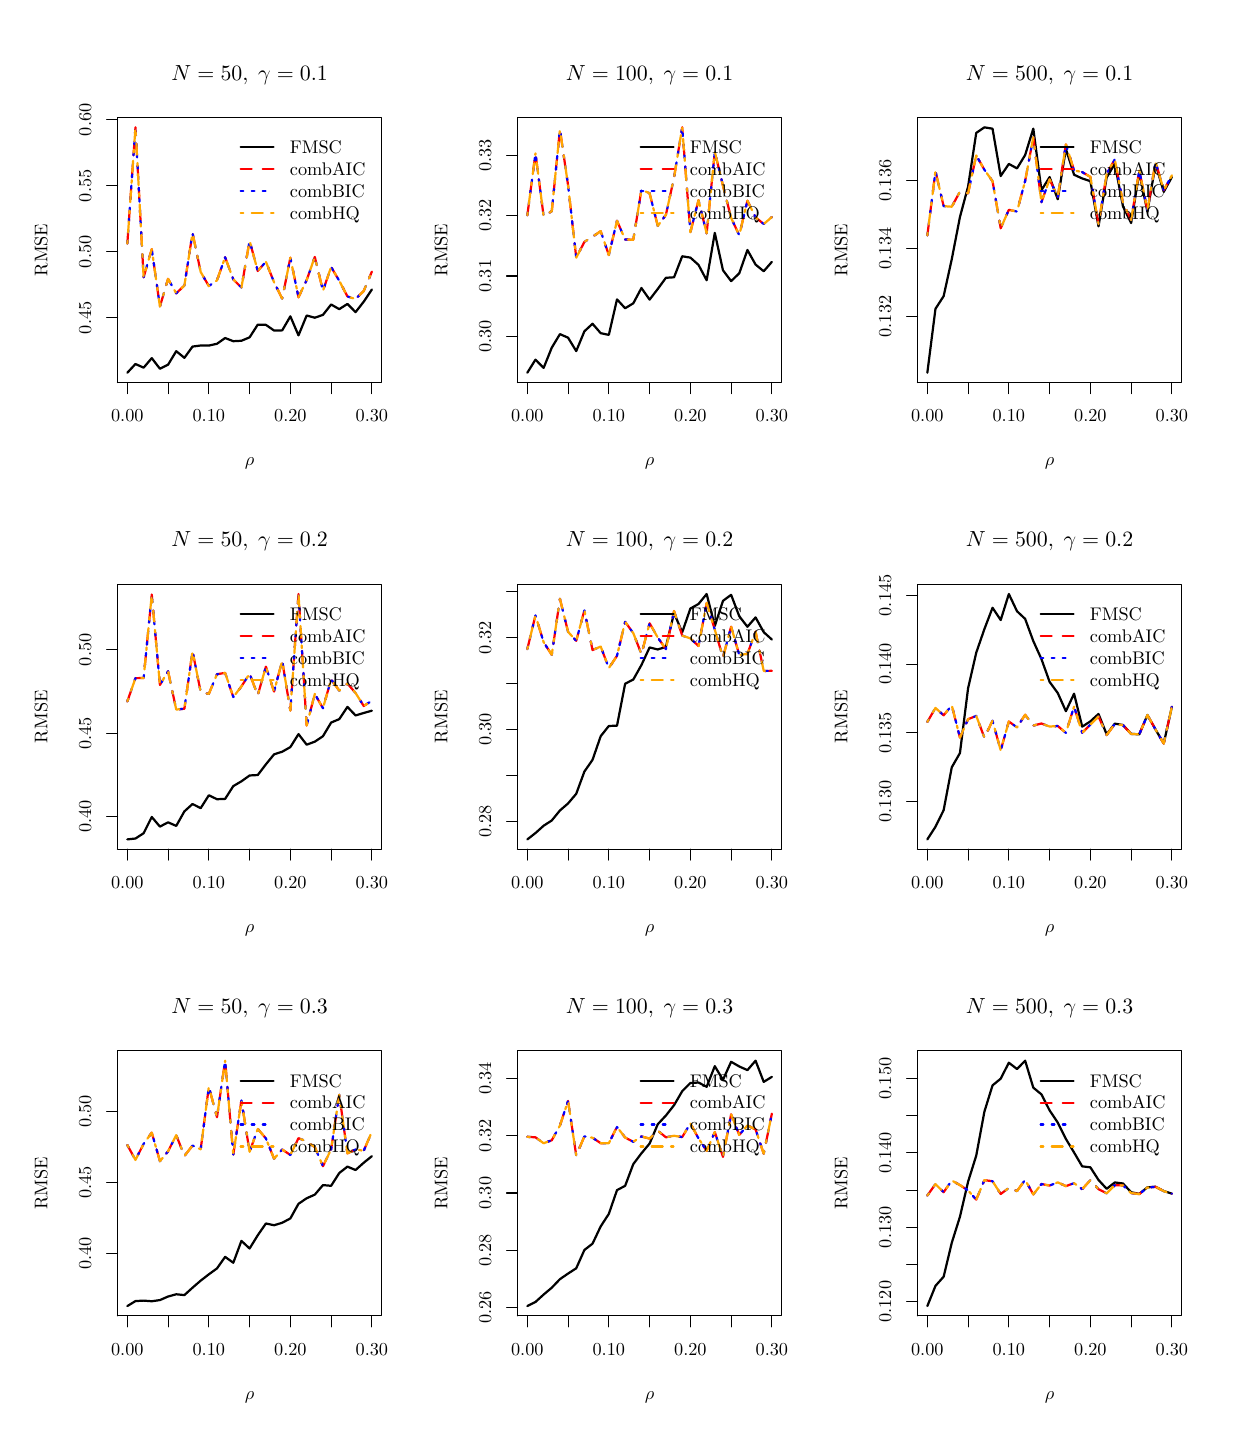
\begin{tikzpicture}[x=1pt,y=1pt]
\definecolor[named]{fillColor}{rgb}{1.00,1.00,1.00}
\path[use as bounding box,fill=fillColor,fill opacity=0.00] (0,0) rectangle (433.62,505.89);
\begin{scope}
\path[clip] ( 32.47,377.65) rectangle (127.91,473.42);
\definecolor[named]{drawColor}{rgb}{0.00,0.00,0.00}

\path[draw=drawColor,line width= 0.8pt,line join=round,line cap=round] ( 36.01,381.20) --
	( 38.95,384.35) --
	( 41.90,383.03) --
	( 44.84,386.48) --
	( 47.79,382.63) --
	( 50.73,384.10) --
	( 53.68,388.99) --
	( 56.63,386.58) --
	( 59.57,390.65) --
	( 62.52,391.04) --
	( 65.46,391.01) --
	( 68.41,391.66) --
	( 71.35,393.74) --
	( 74.30,392.59) --
	( 77.24,392.75) --
	( 80.19,393.98) --
	( 83.14,398.58) --
	( 86.08,398.50) --
	( 89.03,396.45) --
	( 91.97,396.50) --
	( 94.92,401.57) --
	( 97.86,394.70) --
	(100.81,401.88) --
	(103.75,401.08) --
	(106.70,402.10) --
	(109.65,405.86) --
	(112.59,404.17) --
	(115.54,406.06) --
	(118.48,403.09) --
	(121.43,406.87) --
	(124.37,411.27);
\end{scope}
\begin{scope}
\path[clip] (  0.00,  0.00) rectangle (433.62,505.89);
\definecolor[named]{drawColor}{rgb}{0.00,0.00,0.00}

\path[draw=drawColor,line width= 0.4pt,line join=round,line cap=round] ( 36.01,377.65) -- (124.37,377.65);

\path[draw=drawColor,line width= 0.4pt,line join=round,line cap=round] ( 36.01,377.65) -- ( 36.01,373.69);

\path[draw=drawColor,line width= 0.4pt,line join=round,line cap=round] ( 50.73,377.65) -- ( 50.73,373.69);

\path[draw=drawColor,line width= 0.4pt,line join=round,line cap=round] ( 65.46,377.65) -- ( 65.46,373.69);

\path[draw=drawColor,line width= 0.4pt,line join=round,line cap=round] ( 80.19,377.65) -- ( 80.19,373.69);

\path[draw=drawColor,line width= 0.4pt,line join=round,line cap=round] ( 94.92,377.65) -- ( 94.92,373.69);

\path[draw=drawColor,line width= 0.4pt,line join=round,line cap=round] (109.65,377.65) -- (109.65,373.69);

\path[draw=drawColor,line width= 0.4pt,line join=round,line cap=round] (124.37,377.65) -- (124.37,373.69);

\node[text=drawColor,anchor=base,inner sep=0pt, outer sep=0pt, scale=  0.66] at ( 36.01,363.40) {0.00};

\node[text=drawColor,anchor=base,inner sep=0pt, outer sep=0pt, scale=  0.66] at ( 65.46,363.40) {0.10};

\node[text=drawColor,anchor=base,inner sep=0pt, outer sep=0pt, scale=  0.66] at ( 94.92,363.40) {0.20};

\node[text=drawColor,anchor=base,inner sep=0pt, outer sep=0pt, scale=  0.66] at (124.37,363.40) {0.30};

\path[draw=drawColor,line width= 0.4pt,line join=round,line cap=round] ( 32.47,401.06) -- ( 32.47,472.57);

\path[draw=drawColor,line width= 0.4pt,line join=round,line cap=round] ( 32.47,401.06) -- ( 28.51,401.06);

\path[draw=drawColor,line width= 0.4pt,line join=round,line cap=round] ( 32.47,424.90) -- ( 28.51,424.90);

\path[draw=drawColor,line width= 0.4pt,line join=round,line cap=round] ( 32.47,448.74) -- ( 28.51,448.74);

\path[draw=drawColor,line width= 0.4pt,line join=round,line cap=round] ( 32.47,472.57) -- ( 28.51,472.57);

\node[text=drawColor,rotate= 90.00,anchor=base,inner sep=0pt, outer sep=0pt, scale=  0.66] at ( 22.97,401.06) {0.45};

\node[text=drawColor,rotate= 90.00,anchor=base,inner sep=0pt, outer sep=0pt, scale=  0.66] at ( 22.97,424.90) {0.50};

\node[text=drawColor,rotate= 90.00,anchor=base,inner sep=0pt, outer sep=0pt, scale=  0.66] at ( 22.97,448.74) {0.55};

\node[text=drawColor,rotate= 90.00,anchor=base,inner sep=0pt, outer sep=0pt, scale=  0.66] at ( 22.97,472.57) {0.60};

\path[draw=drawColor,line width= 0.4pt,line join=round,line cap=round] ( 32.47,377.65) --
	(127.91,377.65) --
	(127.91,473.42) --
	( 32.47,473.42) --
	( 32.47,377.65);
\end{scope}
\begin{scope}
\path[clip] (  0.00,337.26) rectangle (144.54,505.89);
\definecolor[named]{drawColor}{rgb}{0.00,0.00,0.00}

\node[text=drawColor,anchor=base,inner sep=0pt, outer sep=0pt, scale=  0.79] at ( 80.19,486.92) {\bfseries $N=50, \;\gamma=0.1$};

\node[text=drawColor,anchor=base,inner sep=0pt, outer sep=0pt, scale=  0.66] at ( 80.19,347.56) {$\rho$};

\node[text=drawColor,rotate= 90.00,anchor=base,inner sep=0pt, outer sep=0pt, scale=  0.66] at (  7.13,425.53) {RMSE};
\end{scope}
\begin{scope}
\path[clip] ( 32.47,377.65) rectangle (127.91,473.42);
\definecolor[named]{drawColor}{rgb}{1.00,0.00,0.00}

\path[draw=drawColor,line width= 0.8pt,dash pattern=on 4pt off 4pt ,line join=round,line cap=round] ( 36.01,427.87) --
	( 38.95,469.87) --
	( 41.90,415.68) --
	( 44.84,425.86) --
	( 47.79,405.13) --
	( 50.73,415.13) --
	( 53.68,409.90) --
	( 56.63,412.72) --
	( 59.57,431.68) --
	( 62.52,417.61) --
	( 65.46,412.52) --
	( 68.41,414.58) --
	( 71.35,422.92) --
	( 74.30,414.92) --
	( 77.24,411.96) --
	( 80.19,428.89) --
	( 83.14,417.98) --
	( 86.08,421.30) --
	( 89.03,413.91) --
	( 91.97,407.95) --
	( 94.92,422.75) --
	( 97.86,408.47) --
	(100.81,414.67) --
	(103.75,423.05) --
	(106.70,410.80) --
	(109.65,419.41) --
	(112.59,414.42) --
	(115.54,408.77) --
	(118.48,407.81) --
	(121.43,410.74) --
	(124.37,417.73);
\definecolor[named]{drawColor}{rgb}{0.00,0.00,1.00}

\path[draw=drawColor,line width= 0.8pt,dash pattern=on 1pt off 3pt ,line join=round,line cap=round] ( 36.01,427.87) --
	( 38.95,469.87) --
	( 41.90,415.68) --
	( 44.84,425.86) --
	( 47.79,405.13) --
	( 50.73,415.13) --
	( 53.68,409.90) --
	( 56.63,412.72) --
	( 59.57,431.68) --
	( 62.52,417.61) --
	( 65.46,412.52) --
	( 68.41,414.58) --
	( 71.35,422.92) --
	( 74.30,414.92) --
	( 77.24,411.96) --
	( 80.19,428.89) --
	( 83.14,417.98) --
	( 86.08,421.30) --
	( 89.03,413.91) --
	( 91.97,407.95) --
	( 94.92,422.75) --
	( 97.86,408.47) --
	(100.81,414.67) --
	(103.75,423.05) --
	(106.70,410.80) --
	(109.65,419.41) --
	(112.59,414.42) --
	(115.54,408.77) --
	(118.48,407.81) --
	(121.43,410.74) --
	(124.37,417.73);
\definecolor[named]{drawColor}{rgb}{1.00,0.65,0.00}

\path[draw=drawColor,line width= 0.8pt,dash pattern=on 1pt off 3pt on 4pt off 3pt ,line join=round,line cap=round] ( 36.01,427.87) --
	( 38.95,469.87) --
	( 41.90,415.68) --
	( 44.84,425.86) --
	( 47.79,405.13) --
	( 50.73,415.13) --
	( 53.68,409.90) --
	( 56.63,412.72) --
	( 59.57,431.68) --
	( 62.52,417.61) --
	( 65.46,412.52) --
	( 68.41,414.58) --
	( 71.35,422.92) --
	( 74.30,414.92) --
	( 77.24,411.96) --
	( 80.19,428.89) --
	( 83.14,417.98) --
	( 86.08,421.30) --
	( 89.03,413.91) --
	( 91.97,407.95) --
	( 94.92,422.75) --
	( 97.86,408.47) --
	(100.81,414.67) --
	(103.75,423.05) --
	(106.70,410.80) --
	(109.65,419.41) --
	(112.59,414.42) --
	(115.54,408.77) --
	(118.48,407.81) --
	(121.43,410.74) --
	(124.37,417.73);
\definecolor[named]{drawColor}{rgb}{0.00,0.00,0.00}

\path[draw=drawColor,line width= 0.8pt,line join=round,line cap=round] ( 76.94,462.63) -- ( 88.82,462.63);
\definecolor[named]{drawColor}{rgb}{1.00,0.00,0.00}

\path[draw=drawColor,line width= 0.8pt,dash pattern=on 4pt off 4pt ,line join=round,line cap=round] ( 76.94,454.71) -- ( 88.82,454.71);
\definecolor[named]{drawColor}{rgb}{0.00,0.00,1.00}

\path[draw=drawColor,line width= 0.8pt,dash pattern=on 1pt off 3pt ,line join=round,line cap=round] ( 76.94,446.79) -- ( 88.82,446.79);
\definecolor[named]{drawColor}{rgb}{1.00,0.65,0.00}

\path[draw=drawColor,line width= 0.8pt,dash pattern=on 1pt off 3pt on 4pt off 3pt ,line join=round,line cap=round] ( 76.94,438.87) -- ( 88.82,438.87);
\definecolor[named]{drawColor}{rgb}{0.00,0.00,0.00}

\node[text=drawColor,anchor=base west,inner sep=0pt, outer sep=0pt, scale=  0.66] at ( 94.76,460.35) {FMSC};

\node[text=drawColor,anchor=base west,inner sep=0pt, outer sep=0pt, scale=  0.66] at ( 94.76,452.43) {combAIC};

\node[text=drawColor,anchor=base west,inner sep=0pt, outer sep=0pt, scale=  0.66] at ( 94.76,444.51) {combBIC};

\node[text=drawColor,anchor=base west,inner sep=0pt, outer sep=0pt, scale=  0.66] at ( 94.76,436.59) {combHQ};
\end{scope}
\begin{scope}
\path[clip] (177.01,377.65) rectangle (272.45,473.42);
\definecolor[named]{drawColor}{rgb}{0.00,0.00,0.00}

\path[draw=drawColor,line width= 0.8pt,line join=round,line cap=round] (180.55,381.20) --
	(183.49,385.93) --
	(186.44,382.95) --
	(189.38,390.26) --
	(192.33,395.15) --
	(195.27,393.86) --
	(198.22,389.02) --
	(201.17,396.17) --
	(204.11,398.90) --
	(207.06,395.49) --
	(210.00,394.87) --
	(212.95,407.70) --
	(215.89,404.50) --
	(218.84,406.28) --
	(221.78,411.81) --
	(224.73,407.62) --
	(227.68,411.46) --
	(230.62,415.50) --
	(233.57,415.69) --
	(236.51,423.28) --
	(239.46,422.80) --
	(242.40,420.17) --
	(245.35,414.61) --
	(248.29,431.74) --
	(251.24,418.23) --
	(254.19,414.30) --
	(257.13,417.13) --
	(260.08,425.56) --
	(263.02,420.28) --
	(265.97,417.87) --
	(268.91,421.26);
\end{scope}
\begin{scope}
\path[clip] (  0.00,  0.00) rectangle (433.62,505.89);
\definecolor[named]{drawColor}{rgb}{0.00,0.00,0.00}

\path[draw=drawColor,line width= 0.4pt,line join=round,line cap=round] (180.55,377.65) -- (268.91,377.65);

\path[draw=drawColor,line width= 0.4pt,line join=round,line cap=round] (180.55,377.65) -- (180.55,373.69);

\path[draw=drawColor,line width= 0.4pt,line join=round,line cap=round] (195.27,377.65) -- (195.27,373.69);

\path[draw=drawColor,line width= 0.4pt,line join=round,line cap=round] (210.00,377.65) -- (210.00,373.69);

\path[draw=drawColor,line width= 0.4pt,line join=round,line cap=round] (224.73,377.65) -- (224.73,373.69);

\path[draw=drawColor,line width= 0.4pt,line join=round,line cap=round] (239.46,377.65) -- (239.46,373.69);

\path[draw=drawColor,line width= 0.4pt,line join=round,line cap=round] (254.19,377.65) -- (254.19,373.69);

\path[draw=drawColor,line width= 0.4pt,line join=round,line cap=round] (268.91,377.65) -- (268.91,373.69);

\node[text=drawColor,anchor=base,inner sep=0pt, outer sep=0pt, scale=  0.66] at (180.55,363.40) {0.00};

\node[text=drawColor,anchor=base,inner sep=0pt, outer sep=0pt, scale=  0.66] at (210.00,363.40) {0.10};

\node[text=drawColor,anchor=base,inner sep=0pt, outer sep=0pt, scale=  0.66] at (239.46,363.40) {0.20};

\node[text=drawColor,anchor=base,inner sep=0pt, outer sep=0pt, scale=  0.66] at (268.91,363.40) {0.30};

\path[draw=drawColor,line width= 0.4pt,line join=round,line cap=round] (177.01,394.38) -- (177.01,459.73);

\path[draw=drawColor,line width= 0.4pt,line join=round,line cap=round] (177.01,394.38) -- (173.05,394.38);

\path[draw=drawColor,line width= 0.4pt,line join=round,line cap=round] (177.01,416.16) -- (173.05,416.16);

\path[draw=drawColor,line width= 0.4pt,line join=round,line cap=round] (177.01,437.95) -- (173.05,437.95);

\path[draw=drawColor,line width= 0.4pt,line join=round,line cap=round] (177.01,459.73) -- (173.05,459.73);

\node[text=drawColor,rotate= 90.00,anchor=base,inner sep=0pt, outer sep=0pt, scale=  0.66] at (167.51,394.38) {0.30};

\node[text=drawColor,rotate= 90.00,anchor=base,inner sep=0pt, outer sep=0pt, scale=  0.66] at (167.51,416.16) {0.31};

\node[text=drawColor,rotate= 90.00,anchor=base,inner sep=0pt, outer sep=0pt, scale=  0.66] at (167.51,437.95) {0.32};

\node[text=drawColor,rotate= 90.00,anchor=base,inner sep=0pt, outer sep=0pt, scale=  0.66] at (167.51,459.73) {0.33};

\path[draw=drawColor,line width= 0.4pt,line join=round,line cap=round] (177.01,377.65) --
	(272.45,377.65) --
	(272.45,473.42) --
	(177.01,473.42) --
	(177.01,377.65);
\end{scope}
\begin{scope}
\path[clip] (144.54,337.26) rectangle (289.08,505.89);
\definecolor[named]{drawColor}{rgb}{0.00,0.00,0.00}

\node[text=drawColor,anchor=base,inner sep=0pt, outer sep=0pt, scale=  0.79] at (224.73,486.92) {\bfseries $N=100, \;\gamma=0.1$};

\node[text=drawColor,anchor=base,inner sep=0pt, outer sep=0pt, scale=  0.66] at (224.73,347.56) {$\rho$};

\node[text=drawColor,rotate= 90.00,anchor=base,inner sep=0pt, outer sep=0pt, scale=  0.66] at (151.67,425.53) {RMSE};
\end{scope}
\begin{scope}
\path[clip] (177.01,377.65) rectangle (272.45,473.42);
\definecolor[named]{drawColor}{rgb}{1.00,0.00,0.00}

\path[draw=drawColor,line width= 0.8pt,dash pattern=on 4pt off 4pt ,line join=round,line cap=round] (180.55,438.09) --
	(183.49,460.46) --
	(186.44,437.75) --
	(189.38,439.57) --
	(192.33,469.10) --
	(195.27,448.94) --
	(198.22,422.77) --
	(201.17,428.48) --
	(204.11,430.35) --
	(207.06,432.35) --
	(210.00,423.70) --
	(212.95,436.10) --
	(215.89,429.35) --
	(218.84,429.26) --
	(221.78,447.34) --
	(224.73,446.05) --
	(227.68,434.24) --
	(230.62,438.25) --
	(233.57,451.72) --
	(236.51,469.87) --
	(239.46,431.96) --
	(242.40,443.55) --
	(245.35,431.57) --
	(248.29,461.07) --
	(251.24,448.81) --
	(254.19,437.14) --
	(257.13,430.87) --
	(260.08,443.36) --
	(263.02,437.35) --
	(265.97,434.93) --
	(268.91,437.45);
\definecolor[named]{drawColor}{rgb}{0.00,0.00,1.00}

\path[draw=drawColor,line width= 0.8pt,dash pattern=on 1pt off 3pt ,line join=round,line cap=round] (180.55,438.09) --
	(183.49,460.46) --
	(186.44,437.75) --
	(189.38,439.57) --
	(192.33,469.10) --
	(195.27,448.94) --
	(198.22,422.77) --
	(201.17,428.48) --
	(204.11,430.35) --
	(207.06,432.35) --
	(210.00,423.70) --
	(212.95,436.10) --
	(215.89,429.35) --
	(218.84,429.26) --
	(221.78,447.34) --
	(224.73,446.05) --
	(227.68,434.24) --
	(230.62,438.25) --
	(233.57,451.72) --
	(236.51,469.87) --
	(239.46,431.96) --
	(242.40,443.55) --
	(245.35,431.57) --
	(248.29,461.07) --
	(251.24,448.81) --
	(254.19,437.14) --
	(257.13,430.87) --
	(260.08,443.36) --
	(263.02,437.35) --
	(265.97,434.93) --
	(268.91,437.45);
\definecolor[named]{drawColor}{rgb}{1.00,0.65,0.00}

\path[draw=drawColor,line width= 0.8pt,dash pattern=on 1pt off 3pt on 4pt off 3pt ,line join=round,line cap=round] (180.55,438.09) --
	(183.49,460.46) --
	(186.44,437.75) --
	(189.38,439.57) --
	(192.33,469.10) --
	(195.27,448.94) --
	(198.22,422.77) --
	(201.17,428.48) --
	(204.11,430.35) --
	(207.06,432.35) --
	(210.00,423.70) --
	(212.95,436.10) --
	(215.89,429.35) --
	(218.84,429.26) --
	(221.78,447.34) --
	(224.73,446.05) --
	(227.68,434.24) --
	(230.62,438.25) --
	(233.57,451.72) --
	(236.51,469.87) --
	(239.46,431.96) --
	(242.40,443.55) --
	(245.35,431.57) --
	(248.29,461.07) --
	(251.24,448.81) --
	(254.19,437.14) --
	(257.13,430.87) --
	(260.08,443.36) --
	(263.02,437.35) --
	(265.97,434.93) --
	(268.91,437.45);
\definecolor[named]{drawColor}{rgb}{0.00,0.00,0.00}

\path[draw=drawColor,line width= 0.8pt,line join=round,line cap=round] (221.48,462.63) -- (233.36,462.63);
\definecolor[named]{drawColor}{rgb}{1.00,0.00,0.00}

\path[draw=drawColor,line width= 0.8pt,dash pattern=on 4pt off 4pt ,line join=round,line cap=round] (221.48,454.71) -- (233.36,454.71);
\definecolor[named]{drawColor}{rgb}{0.00,0.00,1.00}

\path[draw=drawColor,line width= 0.8pt,dash pattern=on 1pt off 3pt ,line join=round,line cap=round] (221.48,446.79) -- (233.36,446.79);
\definecolor[named]{drawColor}{rgb}{1.00,0.65,0.00}

\path[draw=drawColor,line width= 0.8pt,dash pattern=on 1pt off 3pt on 4pt off 3pt ,line join=round,line cap=round] (221.48,438.87) -- (233.36,438.87);
\definecolor[named]{drawColor}{rgb}{0.00,0.00,0.00}

\node[text=drawColor,anchor=base west,inner sep=0pt, outer sep=0pt, scale=  0.66] at (239.30,460.35) {FMSC};

\node[text=drawColor,anchor=base west,inner sep=0pt, outer sep=0pt, scale=  0.66] at (239.30,452.43) {combAIC};

\node[text=drawColor,anchor=base west,inner sep=0pt, outer sep=0pt, scale=  0.66] at (239.30,444.51) {combBIC};

\node[text=drawColor,anchor=base west,inner sep=0pt, outer sep=0pt, scale=  0.66] at (239.30,436.59) {combHQ};
\end{scope}
\begin{scope}
\path[clip] (321.55,377.65) rectangle (416.99,473.42);
\definecolor[named]{drawColor}{rgb}{0.00,0.00,0.00}

\path[draw=drawColor,line width= 0.8pt,line join=round,line cap=round] (325.09,381.20) --
	(328.03,404.30) --
	(330.98,408.87) --
	(333.92,422.24) --
	(336.87,437.45) --
	(339.81,448.46) --
	(342.76,467.85) --
	(345.71,469.87) --
	(348.65,469.38) --
	(351.60,452.27) --
	(354.54,456.66) --
	(357.49,455.04) --
	(360.43,459.85) --
	(363.38,469.41) --
	(366.32,447.13) --
	(369.27,451.89) --
	(372.22,443.88) --
	(375.16,462.07) --
	(378.11,452.74) --
	(381.05,451.40) --
	(384.00,450.42) --
	(386.94,434.09) --
	(389.89,451.76) --
	(392.83,456.70) --
	(395.78,441.36) --
	(398.73,435.28) --
	(401.67,453.60) --
	(404.62,439.35) --
	(407.56,456.62) --
	(410.51,446.55) --
	(413.45,451.91);
\end{scope}
\begin{scope}
\path[clip] (  0.00,  0.00) rectangle (433.62,505.89);
\definecolor[named]{drawColor}{rgb}{0.00,0.00,0.00}

\path[draw=drawColor,line width= 0.4pt,line join=round,line cap=round] (325.09,377.65) -- (413.45,377.65);

\path[draw=drawColor,line width= 0.4pt,line join=round,line cap=round] (325.09,377.65) -- (325.09,373.69);

\path[draw=drawColor,line width= 0.4pt,line join=round,line cap=round] (339.81,377.65) -- (339.81,373.69);

\path[draw=drawColor,line width= 0.4pt,line join=round,line cap=round] (354.54,377.65) -- (354.54,373.69);

\path[draw=drawColor,line width= 0.4pt,line join=round,line cap=round] (369.27,377.65) -- (369.27,373.69);

\path[draw=drawColor,line width= 0.4pt,line join=round,line cap=round] (384.00,377.65) -- (384.00,373.69);

\path[draw=drawColor,line width= 0.4pt,line join=round,line cap=round] (398.73,377.65) -- (398.73,373.69);

\path[draw=drawColor,line width= 0.4pt,line join=round,line cap=round] (413.45,377.65) -- (413.45,373.69);

\node[text=drawColor,anchor=base,inner sep=0pt, outer sep=0pt, scale=  0.66] at (325.09,363.40) {0.00};

\node[text=drawColor,anchor=base,inner sep=0pt, outer sep=0pt, scale=  0.66] at (354.54,363.40) {0.10};

\node[text=drawColor,anchor=base,inner sep=0pt, outer sep=0pt, scale=  0.66] at (384.00,363.40) {0.20};

\node[text=drawColor,anchor=base,inner sep=0pt, outer sep=0pt, scale=  0.66] at (413.45,363.40) {0.30};

\path[draw=drawColor,line width= 0.4pt,line join=round,line cap=round] (321.55,401.51) -- (321.55,450.69);

\path[draw=drawColor,line width= 0.4pt,line join=round,line cap=round] (321.55,401.51) -- (317.59,401.51);

\path[draw=drawColor,line width= 0.4pt,line join=round,line cap=round] (321.55,426.10) -- (317.59,426.10);

\path[draw=drawColor,line width= 0.4pt,line join=round,line cap=round] (321.55,450.69) -- (317.59,450.69);

\node[text=drawColor,rotate= 90.00,anchor=base,inner sep=0pt, outer sep=0pt, scale=  0.66] at (312.05,401.51) {0.132};

\node[text=drawColor,rotate= 90.00,anchor=base,inner sep=0pt, outer sep=0pt, scale=  0.66] at (312.05,426.10) {0.134};

\node[text=drawColor,rotate= 90.00,anchor=base,inner sep=0pt, outer sep=0pt, scale=  0.66] at (312.05,450.69) {0.136};

\path[draw=drawColor,line width= 0.4pt,line join=round,line cap=round] (321.55,377.65) --
	(416.99,377.65) --
	(416.99,473.42) --
	(321.55,473.42) --
	(321.55,377.65);
\end{scope}
\begin{scope}
\path[clip] (289.08,337.26) rectangle (433.62,505.89);
\definecolor[named]{drawColor}{rgb}{0.00,0.00,0.00}

\node[text=drawColor,anchor=base,inner sep=0pt, outer sep=0pt, scale=  0.79] at (369.27,486.92) {\bfseries $N=500, \;\gamma=0.1$};

\node[text=drawColor,anchor=base,inner sep=0pt, outer sep=0pt, scale=  0.66] at (369.27,347.56) {$\rho$};

\node[text=drawColor,rotate= 90.00,anchor=base,inner sep=0pt, outer sep=0pt, scale=  0.66] at (296.21,425.53) {RMSE};
\end{scope}
\begin{scope}
\path[clip] (321.55,377.65) rectangle (416.99,473.42);
\definecolor[named]{drawColor}{rgb}{1.00,0.00,0.00}

\path[draw=drawColor,line width= 0.8pt,dash pattern=on 4pt off 4pt ,line join=round,line cap=round] (325.09,430.82) --
	(328.03,454.01) --
	(330.98,441.39) --
	(333.92,441.19) --
	(336.87,446.64) --
	(339.81,446.02) --
	(342.76,459.73) --
	(345.71,454.53) --
	(348.65,450.42) --
	(351.60,433.40) --
	(354.54,440.07) --
	(357.49,439.44) --
	(360.43,450.49) --
	(363.38,466.31) --
	(366.32,442.82) --
	(369.27,451.08) --
	(372.22,444.76) --
	(375.16,463.70) --
	(378.11,454.33) --
	(381.05,453.69) --
	(384.00,451.97) --
	(386.94,434.94) --
	(389.89,453.01) --
	(392.83,458.33) --
	(395.78,442.57) --
	(398.73,436.40) --
	(401.67,454.27) --
	(404.62,439.99) --
	(407.56,457.41) --
	(410.51,447.14) --
	(413.45,452.52);
\definecolor[named]{drawColor}{rgb}{0.00,0.00,1.00}

\path[draw=drawColor,line width= 0.8pt,dash pattern=on 1pt off 3pt ,line join=round,line cap=round] (325.09,430.82) --
	(328.03,454.01) --
	(330.98,441.39) --
	(333.92,441.19) --
	(336.87,446.64) --
	(339.81,446.02) --
	(342.76,459.73) --
	(345.71,454.53) --
	(348.65,450.42) --
	(351.60,433.40) --
	(354.54,440.07) --
	(357.49,439.44) --
	(360.43,450.49) --
	(363.38,466.31) --
	(366.32,442.82) --
	(369.27,451.08) --
	(372.22,444.76) --
	(375.16,463.70) --
	(378.11,454.33) --
	(381.05,453.69) --
	(384.00,451.97) --
	(386.94,434.94) --
	(389.89,453.01) --
	(392.83,458.33) --
	(395.78,442.57) --
	(398.73,436.40) --
	(401.67,454.27) --
	(404.62,439.99) --
	(407.56,457.41) --
	(410.51,447.14) --
	(413.45,452.52);
\definecolor[named]{drawColor}{rgb}{1.00,0.65,0.00}

\path[draw=drawColor,line width= 0.8pt,dash pattern=on 1pt off 3pt on 4pt off 3pt ,line join=round,line cap=round] (325.09,430.82) --
	(328.03,454.01) --
	(330.98,441.39) --
	(333.92,441.19) --
	(336.87,446.64) --
	(339.81,446.02) --
	(342.76,459.73) --
	(345.71,454.53) --
	(348.65,450.42) --
	(351.60,433.40) --
	(354.54,440.07) --
	(357.49,439.44) --
	(360.43,450.49) --
	(363.38,466.31) --
	(366.32,442.82) --
	(369.27,451.08) --
	(372.22,444.76) --
	(375.16,463.70) --
	(378.11,454.33) --
	(381.05,453.69) --
	(384.00,451.97) --
	(386.94,434.94) --
	(389.89,453.01) --
	(392.83,458.33) --
	(395.78,442.57) --
	(398.73,436.40) --
	(401.67,454.27) --
	(404.62,439.99) --
	(407.56,457.41) --
	(410.51,447.14) --
	(413.45,452.52);
\definecolor[named]{drawColor}{rgb}{0.00,0.00,0.00}

\path[draw=drawColor,line width= 0.8pt,line join=round,line cap=round] (366.02,462.63) -- (377.90,462.63);
\definecolor[named]{drawColor}{rgb}{1.00,0.00,0.00}

\path[draw=drawColor,line width= 0.8pt,dash pattern=on 4pt off 4pt ,line join=round,line cap=round] (366.02,454.71) -- (377.90,454.71);
\definecolor[named]{drawColor}{rgb}{0.00,0.00,1.00}

\path[draw=drawColor,line width= 0.8pt,dash pattern=on 1pt off 3pt ,line join=round,line cap=round] (366.02,446.79) -- (377.90,446.79);
\definecolor[named]{drawColor}{rgb}{1.00,0.65,0.00}

\path[draw=drawColor,line width= 0.8pt,dash pattern=on 1pt off 3pt on 4pt off 3pt ,line join=round,line cap=round] (366.02,438.87) -- (377.90,438.87);
\definecolor[named]{drawColor}{rgb}{0.00,0.00,0.00}

\node[text=drawColor,anchor=base west,inner sep=0pt, outer sep=0pt, scale=  0.66] at (383.84,460.35) {FMSC};

\node[text=drawColor,anchor=base west,inner sep=0pt, outer sep=0pt, scale=  0.66] at (383.84,452.43) {combAIC};

\node[text=drawColor,anchor=base west,inner sep=0pt, outer sep=0pt, scale=  0.66] at (383.84,444.51) {combBIC};

\node[text=drawColor,anchor=base west,inner sep=0pt, outer sep=0pt, scale=  0.66] at (383.84,436.59) {combHQ};
\end{scope}
\begin{scope}
\path[clip] ( 32.47,209.02) rectangle (127.91,304.79);
\definecolor[named]{drawColor}{rgb}{0.00,0.00,0.00}

\path[draw=drawColor,line width= 0.8pt,line join=round,line cap=round] ( 36.01,212.57) --
	( 38.95,212.89) --
	( 41.90,214.80) --
	( 44.84,220.67) --
	( 47.79,217.19) --
	( 50.73,218.74) --
	( 53.68,217.45) --
	( 56.63,222.70) --
	( 59.57,225.36) --
	( 62.52,223.87) --
	( 65.46,228.51) --
	( 68.41,227.09) --
	( 71.35,227.21) --
	( 74.30,231.83) --
	( 77.24,233.56) --
	( 80.19,235.67) --
	( 83.14,235.83) --
	( 86.08,239.69) --
	( 89.03,243.30) --
	( 91.97,244.26) --
	( 94.92,245.92) --
	( 97.86,250.62) --
	(100.81,246.79) --
	(103.75,247.89) --
	(106.70,249.86) --
	(109.65,254.79) --
	(112.59,256.03) --
	(115.54,260.46) --
	(118.48,257.36) --
	(121.43,258.25) --
	(124.37,259.08);
\end{scope}
\begin{scope}
\path[clip] (  0.00,  0.00) rectangle (433.62,505.89);
\definecolor[named]{drawColor}{rgb}{0.00,0.00,0.00}

\path[draw=drawColor,line width= 0.4pt,line join=round,line cap=round] ( 36.01,209.02) -- (124.37,209.02);

\path[draw=drawColor,line width= 0.4pt,line join=round,line cap=round] ( 36.01,209.02) -- ( 36.01,205.06);

\path[draw=drawColor,line width= 0.4pt,line join=round,line cap=round] ( 50.73,209.02) -- ( 50.73,205.06);

\path[draw=drawColor,line width= 0.4pt,line join=round,line cap=round] ( 65.46,209.02) -- ( 65.46,205.06);

\path[draw=drawColor,line width= 0.4pt,line join=round,line cap=round] ( 80.19,209.02) -- ( 80.19,205.06);

\path[draw=drawColor,line width= 0.4pt,line join=round,line cap=round] ( 94.92,209.02) -- ( 94.92,205.06);

\path[draw=drawColor,line width= 0.4pt,line join=round,line cap=round] (109.65,209.02) -- (109.65,205.06);

\path[draw=drawColor,line width= 0.4pt,line join=round,line cap=round] (124.37,209.02) -- (124.37,205.06);

\node[text=drawColor,anchor=base,inner sep=0pt, outer sep=0pt, scale=  0.66] at ( 36.01,194.77) {0.00};

\node[text=drawColor,anchor=base,inner sep=0pt, outer sep=0pt, scale=  0.66] at ( 65.46,194.77) {0.10};

\node[text=drawColor,anchor=base,inner sep=0pt, outer sep=0pt, scale=  0.66] at ( 94.92,194.77) {0.20};

\node[text=drawColor,anchor=base,inner sep=0pt, outer sep=0pt, scale=  0.66] at (124.37,194.77) {0.30};

\path[draw=drawColor,line width= 0.4pt,line join=round,line cap=round] ( 32.47,220.80) -- ( 32.47,281.08);

\path[draw=drawColor,line width= 0.4pt,line join=round,line cap=round] ( 32.47,220.80) -- ( 28.51,220.80);

\path[draw=drawColor,line width= 0.4pt,line join=round,line cap=round] ( 32.47,250.94) -- ( 28.51,250.94);

\path[draw=drawColor,line width= 0.4pt,line join=round,line cap=round] ( 32.47,281.08) -- ( 28.51,281.08);

\node[text=drawColor,rotate= 90.00,anchor=base,inner sep=0pt, outer sep=0pt, scale=  0.66] at ( 22.97,220.80) {0.40};

\node[text=drawColor,rotate= 90.00,anchor=base,inner sep=0pt, outer sep=0pt, scale=  0.66] at ( 22.97,250.94) {0.45};

\node[text=drawColor,rotate= 90.00,anchor=base,inner sep=0pt, outer sep=0pt, scale=  0.66] at ( 22.97,281.08) {0.50};

\path[draw=drawColor,line width= 0.4pt,line join=round,line cap=round] ( 32.47,209.02) --
	(127.91,209.02) --
	(127.91,304.79) --
	( 32.47,304.79) --
	( 32.47,209.02);
\end{scope}
\begin{scope}
\path[clip] (  0.00,168.63) rectangle (144.54,337.26);
\definecolor[named]{drawColor}{rgb}{0.00,0.00,0.00}

\node[text=drawColor,anchor=base,inner sep=0pt, outer sep=0pt, scale=  0.79] at ( 80.19,318.29) {\bfseries $N=50, \;\gamma=0.2$};

\node[text=drawColor,anchor=base,inner sep=0pt, outer sep=0pt, scale=  0.66] at ( 80.19,178.93) {$\rho$};

\node[text=drawColor,rotate= 90.00,anchor=base,inner sep=0pt, outer sep=0pt, scale=  0.66] at (  7.13,256.90) {RMSE};
\end{scope}
\begin{scope}
\path[clip] ( 32.47,209.02) rectangle (127.91,304.79);
\definecolor[named]{drawColor}{rgb}{1.00,0.00,0.00}

\path[draw=drawColor,line width= 0.8pt,dash pattern=on 4pt off 4pt ,line join=round,line cap=round] ( 36.01,262.43) --
	( 38.95,270.84) --
	( 41.90,270.87) --
	( 44.84,301.05) --
	( 47.79,268.39) --
	( 50.73,273.31) --
	( 53.68,259.49) --
	( 56.63,259.79) --
	( 59.57,280.56) --
	( 62.52,265.84) --
	( 65.46,265.14) --
	( 68.41,272.26) --
	( 71.35,272.73) --
	( 74.30,264.01) --
	( 77.24,267.85) --
	( 80.19,272.44) --
	( 83.14,264.69) --
	( 86.08,274.99) --
	( 89.03,266.00) --
	( 91.97,277.11) --
	( 94.92,259.12) --
	( 97.86,301.24) --
	(100.81,253.73) --
	(103.75,265.13) --
	(106.70,259.96) --
	(109.65,270.38) --
	(112.59,266.32) --
	(115.54,268.89) --
	(118.48,265.48) --
	(121.43,260.78) --
	(124.37,262.67);
\definecolor[named]{drawColor}{rgb}{0.00,0.00,1.00}

\path[draw=drawColor,line width= 0.8pt,dash pattern=on 1pt off 3pt ,line join=round,line cap=round] ( 36.01,262.43) --
	( 38.95,270.84) --
	( 41.90,270.87) --
	( 44.84,301.05) --
	( 47.79,268.39) --
	( 50.73,273.31) --
	( 53.68,259.49) --
	( 56.63,259.79) --
	( 59.57,280.56) --
	( 62.52,265.84) --
	( 65.46,265.14) --
	( 68.41,272.26) --
	( 71.35,272.73) --
	( 74.30,264.01) --
	( 77.24,267.85) --
	( 80.19,272.44) --
	( 83.14,264.69) --
	( 86.08,274.99) --
	( 89.03,266.00) --
	( 91.97,277.11) --
	( 94.92,259.12) --
	( 97.86,301.24) --
	(100.81,253.73) --
	(103.75,265.13) --
	(106.70,259.96) --
	(109.65,270.38) --
	(112.59,266.32) --
	(115.54,268.89) --
	(118.48,265.48) --
	(121.43,260.78) --
	(124.37,262.67);
\definecolor[named]{drawColor}{rgb}{1.00,0.65,0.00}

\path[draw=drawColor,line width= 0.8pt,dash pattern=on 1pt off 3pt on 4pt off 3pt ,line join=round,line cap=round] ( 36.01,262.43) --
	( 38.95,270.84) --
	( 41.90,270.87) --
	( 44.84,301.05) --
	( 47.79,268.39) --
	( 50.73,273.31) --
	( 53.68,259.49) --
	( 56.63,259.79) --
	( 59.57,280.56) --
	( 62.52,265.84) --
	( 65.46,265.14) --
	( 68.41,272.26) --
	( 71.35,272.73) --
	( 74.30,264.01) --
	( 77.24,267.85) --
	( 80.19,272.44) --
	( 83.14,264.69) --
	( 86.08,274.99) --
	( 89.03,266.00) --
	( 91.97,277.11) --
	( 94.92,259.12) --
	( 97.86,301.24) --
	(100.81,253.73) --
	(103.75,265.13) --
	(106.70,259.96) --
	(109.65,270.38) --
	(112.59,266.32) --
	(115.54,268.89) --
	(118.48,265.48) --
	(121.43,260.78) --
	(124.37,262.67);
\definecolor[named]{drawColor}{rgb}{0.00,0.00,0.00}

\path[draw=drawColor,line width= 0.8pt,line join=round,line cap=round] ( 76.94,294.00) -- ( 88.82,294.00);
\definecolor[named]{drawColor}{rgb}{1.00,0.00,0.00}

\path[draw=drawColor,line width= 0.8pt,dash pattern=on 4pt off 4pt ,line join=round,line cap=round] ( 76.94,286.08) -- ( 88.82,286.08);
\definecolor[named]{drawColor}{rgb}{0.00,0.00,1.00}

\path[draw=drawColor,line width= 0.8pt,dash pattern=on 1pt off 3pt ,line join=round,line cap=round] ( 76.94,278.16) -- ( 88.82,278.16);
\definecolor[named]{drawColor}{rgb}{1.00,0.65,0.00}

\path[draw=drawColor,line width= 0.8pt,dash pattern=on 1pt off 3pt on 4pt off 3pt ,line join=round,line cap=round] ( 76.94,270.24) -- ( 88.82,270.24);
\definecolor[named]{drawColor}{rgb}{0.00,0.00,0.00}

\node[text=drawColor,anchor=base west,inner sep=0pt, outer sep=0pt, scale=  0.66] at ( 94.76,291.72) {FMSC};

\node[text=drawColor,anchor=base west,inner sep=0pt, outer sep=0pt, scale=  0.66] at ( 94.76,283.80) {combAIC};

\node[text=drawColor,anchor=base west,inner sep=0pt, outer sep=0pt, scale=  0.66] at ( 94.76,275.88) {combBIC};

\node[text=drawColor,anchor=base west,inner sep=0pt, outer sep=0pt, scale=  0.66] at ( 94.76,267.96) {combHQ};
\end{scope}
\begin{scope}
\path[clip] (177.01,209.02) rectangle (272.45,304.79);
\definecolor[named]{drawColor}{rgb}{0.00,0.00,0.00}

\path[draw=drawColor,line width= 0.8pt,line join=round,line cap=round] (180.55,212.57) --
	(183.49,214.86) --
	(186.44,217.51) --
	(189.38,219.41) --
	(192.33,223.02) --
	(195.27,225.57) --
	(198.22,229.05) --
	(201.17,237.09) --
	(204.11,241.32) --
	(207.06,249.86) --
	(210.00,253.56) --
	(212.95,253.65) --
	(215.89,268.82) --
	(218.84,270.34) --
	(221.78,275.58) --
	(224.73,281.94) --
	(227.68,281.20) --
	(230.62,282.15) --
	(233.57,294.38) --
	(236.51,287.39) --
	(239.46,295.98) --
	(242.40,297.64) --
	(245.35,301.24) --
	(248.29,289.70) --
	(251.24,298.77) --
	(254.19,300.95) --
	(257.13,293.21) --
	(260.08,289.40) --
	(263.02,292.79) --
	(265.97,287.46) --
	(268.91,284.79);
\end{scope}
\begin{scope}
\path[clip] (  0.00,  0.00) rectangle (433.62,505.89);
\definecolor[named]{drawColor}{rgb}{0.00,0.00,0.00}

\path[draw=drawColor,line width= 0.4pt,line join=round,line cap=round] (180.55,209.02) -- (268.91,209.02);

\path[draw=drawColor,line width= 0.4pt,line join=round,line cap=round] (180.55,209.02) -- (180.55,205.06);

\path[draw=drawColor,line width= 0.4pt,line join=round,line cap=round] (195.27,209.02) -- (195.27,205.06);

\path[draw=drawColor,line width= 0.4pt,line join=round,line cap=round] (210.00,209.02) -- (210.00,205.06);

\path[draw=drawColor,line width= 0.4pt,line join=round,line cap=round] (224.73,209.02) -- (224.73,205.06);

\path[draw=drawColor,line width= 0.4pt,line join=round,line cap=round] (239.46,209.02) -- (239.46,205.06);

\path[draw=drawColor,line width= 0.4pt,line join=round,line cap=round] (254.19,209.02) -- (254.19,205.06);

\path[draw=drawColor,line width= 0.4pt,line join=round,line cap=round] (268.91,209.02) -- (268.91,205.06);

\node[text=drawColor,anchor=base,inner sep=0pt, outer sep=0pt, scale=  0.66] at (180.55,194.77) {0.00};

\node[text=drawColor,anchor=base,inner sep=0pt, outer sep=0pt, scale=  0.66] at (210.00,194.77) {0.10};

\node[text=drawColor,anchor=base,inner sep=0pt, outer sep=0pt, scale=  0.66] at (239.46,194.77) {0.20};

\node[text=drawColor,anchor=base,inner sep=0pt, outer sep=0pt, scale=  0.66] at (268.91,194.77) {0.30};

\path[draw=drawColor,line width= 0.4pt,line join=round,line cap=round] (177.01,218.96) -- (177.01,302.05);

\path[draw=drawColor,line width= 0.4pt,line join=round,line cap=round] (177.01,218.96) -- (173.05,218.96);

\path[draw=drawColor,line width= 0.4pt,line join=round,line cap=round] (177.01,235.58) -- (173.05,235.58);

\path[draw=drawColor,line width= 0.4pt,line join=round,line cap=round] (177.01,252.20) -- (173.05,252.20);

\path[draw=drawColor,line width= 0.4pt,line join=round,line cap=round] (177.01,268.82) -- (173.05,268.82);

\path[draw=drawColor,line width= 0.4pt,line join=round,line cap=round] (177.01,285.43) -- (173.05,285.43);

\path[draw=drawColor,line width= 0.4pt,line join=round,line cap=round] (177.01,302.05) -- (173.05,302.05);

\node[text=drawColor,rotate= 90.00,anchor=base,inner sep=0pt, outer sep=0pt, scale=  0.66] at (167.51,218.96) {0.28};

\node[text=drawColor,rotate= 90.00,anchor=base,inner sep=0pt, outer sep=0pt, scale=  0.66] at (167.51,252.20) {0.30};

\node[text=drawColor,rotate= 90.00,anchor=base,inner sep=0pt, outer sep=0pt, scale=  0.66] at (167.51,285.43) {0.32};

\path[draw=drawColor,line width= 0.4pt,line join=round,line cap=round] (177.01,209.02) --
	(272.45,209.02) --
	(272.45,304.79) --
	(177.01,304.79) --
	(177.01,209.02);
\end{scope}
\begin{scope}
\path[clip] (144.54,168.63) rectangle (289.08,337.26);
\definecolor[named]{drawColor}{rgb}{0.00,0.00,0.00}

\node[text=drawColor,anchor=base,inner sep=0pt, outer sep=0pt, scale=  0.79] at (224.73,318.29) {\bfseries $N=100, \;\gamma=0.2$};

\node[text=drawColor,anchor=base,inner sep=0pt, outer sep=0pt, scale=  0.66] at (224.73,178.93) {$\rho$};

\node[text=drawColor,rotate= 90.00,anchor=base,inner sep=0pt, outer sep=0pt, scale=  0.66] at (151.67,256.90) {RMSE};
\end{scope}
\begin{scope}
\path[clip] (177.01,209.02) rectangle (272.45,304.79);
\definecolor[named]{drawColor}{rgb}{1.00,0.00,0.00}

\path[draw=drawColor,line width= 0.8pt,dash pattern=on 4pt off 4pt ,line join=round,line cap=round] (180.55,281.35) --
	(183.49,293.52) --
	(186.44,283.83) --
	(189.38,279.27) --
	(192.33,299.50) --
	(195.27,287.57) --
	(198.22,284.33) --
	(201.17,295.33) --
	(204.11,281.00) --
	(207.06,282.26) --
	(210.00,274.48) --
	(212.95,278.92) --
	(215.89,291.18) --
	(218.84,287.10) --
	(221.78,279.54) --
	(224.73,290.68) --
	(227.68,285.51) --
	(230.62,281.30) --
	(233.57,295.10) --
	(236.51,286.22) --
	(239.46,285.20) --
	(242.40,282.45) --
	(245.35,298.00) --
	(248.29,288.35) --
	(251.24,278.32) --
	(254.19,289.45) --
	(257.13,279.21) --
	(260.08,279.60) --
	(263.02,287.60) --
	(265.97,273.45) --
	(268.91,273.48);
\definecolor[named]{drawColor}{rgb}{0.00,0.00,1.00}

\path[draw=drawColor,line width= 0.8pt,dash pattern=on 1pt off 3pt ,line join=round,line cap=round] (180.55,281.35) --
	(183.49,293.52) --
	(186.44,283.83) --
	(189.38,279.27) --
	(192.33,299.50) --
	(195.27,287.57) --
	(198.22,284.33) --
	(201.17,295.33) --
	(204.11,281.00) --
	(207.06,282.26) --
	(210.00,274.48) --
	(212.95,278.92) --
	(215.89,291.18) --
	(218.84,287.10) --
	(221.78,279.54) --
	(224.73,290.68) --
	(227.68,285.51) --
	(230.62,281.30) --
	(233.57,295.10) --
	(236.51,286.22) --
	(239.46,285.20) --
	(242.40,282.45) --
	(245.35,298.00) --
	(248.29,288.35) --
	(251.24,278.32) --
	(254.19,289.45) --
	(257.13,279.21) --
	(260.08,279.60) --
	(263.02,287.60) --
	(265.97,273.45) --
	(268.91,273.48);
\definecolor[named]{drawColor}{rgb}{1.00,0.65,0.00}

\path[draw=drawColor,line width= 0.8pt,dash pattern=on 1pt off 3pt on 4pt off 3pt ,line join=round,line cap=round] (180.55,281.35) --
	(183.49,293.52) --
	(186.44,283.83) --
	(189.38,279.27) --
	(192.33,299.50) --
	(195.27,287.57) --
	(198.22,284.33) --
	(201.17,295.33) --
	(204.11,281.00) --
	(207.06,282.26) --
	(210.00,274.48) --
	(212.95,278.92) --
	(215.89,291.18) --
	(218.84,287.10) --
	(221.78,279.54) --
	(224.73,290.68) --
	(227.68,285.51) --
	(230.62,281.30) --
	(233.57,295.10) --
	(236.51,286.22) --
	(239.46,285.20) --
	(242.40,282.45) --
	(245.35,298.00) --
	(248.29,288.35) --
	(251.24,278.32) --
	(254.19,289.45) --
	(257.13,279.21) --
	(260.08,279.60) --
	(263.02,287.60) --
	(265.97,273.45) --
	(268.91,273.48);
\definecolor[named]{drawColor}{rgb}{0.00,0.00,0.00}

\path[draw=drawColor,line width= 0.8pt,line join=round,line cap=round] (221.48,294.00) -- (233.36,294.00);
\definecolor[named]{drawColor}{rgb}{1.00,0.00,0.00}

\path[draw=drawColor,line width= 0.8pt,dash pattern=on 4pt off 4pt ,line join=round,line cap=round] (221.48,286.08) -- (233.36,286.08);
\definecolor[named]{drawColor}{rgb}{0.00,0.00,1.00}

\path[draw=drawColor,line width= 0.8pt,dash pattern=on 1pt off 3pt ,line join=round,line cap=round] (221.48,278.16) -- (233.36,278.16);
\definecolor[named]{drawColor}{rgb}{1.00,0.65,0.00}

\path[draw=drawColor,line width= 0.8pt,dash pattern=on 1pt off 3pt on 4pt off 3pt ,line join=round,line cap=round] (221.48,270.24) -- (233.36,270.24);
\definecolor[named]{drawColor}{rgb}{0.00,0.00,0.00}

\node[text=drawColor,anchor=base west,inner sep=0pt, outer sep=0pt, scale=  0.66] at (239.30,291.72) {FMSC};

\node[text=drawColor,anchor=base west,inner sep=0pt, outer sep=0pt, scale=  0.66] at (239.30,283.80) {combAIC};

\node[text=drawColor,anchor=base west,inner sep=0pt, outer sep=0pt, scale=  0.66] at (239.30,275.88) {combBIC};

\node[text=drawColor,anchor=base west,inner sep=0pt, outer sep=0pt, scale=  0.66] at (239.30,267.96) {combHQ};
\end{scope}
\begin{scope}
\path[clip] (321.55,209.02) rectangle (416.99,304.79);
\definecolor[named]{drawColor}{rgb}{0.00,0.00,0.00}

\path[draw=drawColor,line width= 0.8pt,line join=round,line cap=round] (325.09,212.57) --
	(328.03,217.14) --
	(330.98,223.13) --
	(333.92,238.63) --
	(336.87,243.77) --
	(339.81,267.16) --
	(342.76,280.03) --
	(345.71,288.58) --
	(348.65,296.27) --
	(351.60,291.83) --
	(354.54,301.24) --
	(357.49,295.02) --
	(360.43,292.25) --
	(363.38,284.23) --
	(366.32,277.74) --
	(369.27,269.49) --
	(372.22,265.45) --
	(375.16,258.90) --
	(378.11,265.22) --
	(381.05,253.30) --
	(384.00,255.22) --
	(386.94,257.90) --
	(389.89,250.53) --
	(392.83,254.40) --
	(395.78,253.91) --
	(398.73,250.71) --
	(401.67,250.53) --
	(404.62,257.52) --
	(407.56,252.26) --
	(410.51,247.23) --
	(413.45,260.47);
\end{scope}
\begin{scope}
\path[clip] (  0.00,  0.00) rectangle (433.62,505.89);
\definecolor[named]{drawColor}{rgb}{0.00,0.00,0.00}

\path[draw=drawColor,line width= 0.4pt,line join=round,line cap=round] (325.09,209.02) -- (413.45,209.02);

\path[draw=drawColor,line width= 0.4pt,line join=round,line cap=round] (325.09,209.02) -- (325.09,205.06);

\path[draw=drawColor,line width= 0.4pt,line join=round,line cap=round] (339.81,209.02) -- (339.81,205.06);

\path[draw=drawColor,line width= 0.4pt,line join=round,line cap=round] (354.54,209.02) -- (354.54,205.06);

\path[draw=drawColor,line width= 0.4pt,line join=round,line cap=round] (369.27,209.02) -- (369.27,205.06);

\path[draw=drawColor,line width= 0.4pt,line join=round,line cap=round] (384.00,209.02) -- (384.00,205.06);

\path[draw=drawColor,line width= 0.4pt,line join=round,line cap=round] (398.73,209.02) -- (398.73,205.06);

\path[draw=drawColor,line width= 0.4pt,line join=round,line cap=round] (413.45,209.02) -- (413.45,205.06);

\node[text=drawColor,anchor=base,inner sep=0pt, outer sep=0pt, scale=  0.66] at (325.09,194.77) {0.00};

\node[text=drawColor,anchor=base,inner sep=0pt, outer sep=0pt, scale=  0.66] at (354.54,194.77) {0.10};

\node[text=drawColor,anchor=base,inner sep=0pt, outer sep=0pt, scale=  0.66] at (384.00,194.77) {0.20};

\node[text=drawColor,anchor=base,inner sep=0pt, outer sep=0pt, scale=  0.66] at (413.45,194.77) {0.30};

\path[draw=drawColor,line width= 0.4pt,line join=round,line cap=round] (321.55,226.26) -- (321.55,300.76);

\path[draw=drawColor,line width= 0.4pt,line join=round,line cap=round] (321.55,226.26) -- (317.59,226.26);

\path[draw=drawColor,line width= 0.4pt,line join=round,line cap=round] (321.55,251.10) -- (317.59,251.10);

\path[draw=drawColor,line width= 0.4pt,line join=round,line cap=round] (321.55,275.93) -- (317.59,275.93);

\path[draw=drawColor,line width= 0.4pt,line join=round,line cap=round] (321.55,300.76) -- (317.59,300.76);

\node[text=drawColor,rotate= 90.00,anchor=base,inner sep=0pt, outer sep=0pt, scale=  0.66] at (312.05,226.26) {0.130};

\node[text=drawColor,rotate= 90.00,anchor=base,inner sep=0pt, outer sep=0pt, scale=  0.66] at (312.05,251.10) {0.135};

\node[text=drawColor,rotate= 90.00,anchor=base,inner sep=0pt, outer sep=0pt, scale=  0.66] at (312.05,275.93) {0.140};

\node[text=drawColor,rotate= 90.00,anchor=base,inner sep=0pt, outer sep=0pt, scale=  0.66] at (312.05,300.76) {0.145};

\path[draw=drawColor,line width= 0.4pt,line join=round,line cap=round] (321.55,209.02) --
	(416.99,209.02) --
	(416.99,304.79) --
	(321.55,304.79) --
	(321.55,209.02);
\end{scope}
\begin{scope}
\path[clip] (289.08,168.63) rectangle (433.62,337.26);
\definecolor[named]{drawColor}{rgb}{0.00,0.00,0.00}

\node[text=drawColor,anchor=base,inner sep=0pt, outer sep=0pt, scale=  0.79] at (369.27,318.29) {\bfseries $N=500, \;\gamma=0.2$};

\node[text=drawColor,anchor=base,inner sep=0pt, outer sep=0pt, scale=  0.66] at (369.27,178.93) {$\rho$};

\node[text=drawColor,rotate= 90.00,anchor=base,inner sep=0pt, outer sep=0pt, scale=  0.66] at (296.21,256.90) {RMSE};
\end{scope}
\begin{scope}
\path[clip] (321.55,209.02) rectangle (416.99,304.79);
\definecolor[named]{drawColor}{rgb}{1.00,0.00,0.00}

\path[draw=drawColor,line width= 0.8pt,dash pattern=on 4pt off 4pt ,line join=round,line cap=round] (325.09,255.02) --
	(328.03,260.08) --
	(330.98,257.41) --
	(333.92,261.00) --
	(336.87,249.37) --
	(339.81,256.00) --
	(342.76,257.20) --
	(345.71,249.36) --
	(348.65,255.45) --
	(351.60,244.76) --
	(354.54,255.17) --
	(357.49,253.04) --
	(360.43,257.60) --
	(363.38,253.70) --
	(366.32,254.45) --
	(369.27,253.35) --
	(372.22,253.54) --
	(375.16,251.06) --
	(378.11,260.54) --
	(381.05,251.12) --
	(384.00,254.02) --
	(386.94,256.99) --
	(389.89,250.28) --
	(392.83,254.22) --
	(395.78,253.85) --
	(398.73,250.68) --
	(401.67,250.53) --
	(404.62,257.52) --
	(407.56,252.26) --
	(410.51,247.23) --
	(413.45,260.47);
\definecolor[named]{drawColor}{rgb}{0.00,0.00,1.00}

\path[draw=drawColor,line width= 0.8pt,dash pattern=on 1pt off 3pt ,line join=round,line cap=round] (325.09,255.02) --
	(328.03,260.08) --
	(330.98,257.41) --
	(333.92,261.00) --
	(336.87,249.37) --
	(339.81,256.00) --
	(342.76,257.20) --
	(345.71,249.36) --
	(348.65,255.45) --
	(351.60,244.76) --
	(354.54,255.17) --
	(357.49,253.04) --
	(360.43,257.60) --
	(363.38,253.70) --
	(366.32,254.45) --
	(369.27,253.35) --
	(372.22,253.54) --
	(375.16,251.06) --
	(378.11,260.54) --
	(381.05,251.12) --
	(384.00,254.02) --
	(386.94,256.99) --
	(389.89,250.28) --
	(392.83,254.22) --
	(395.78,253.85) --
	(398.73,250.68) --
	(401.67,250.53) --
	(404.62,257.52) --
	(407.56,252.26) --
	(410.51,247.23) --
	(413.45,260.47);
\definecolor[named]{drawColor}{rgb}{1.00,0.65,0.00}

\path[draw=drawColor,line width= 0.8pt,dash pattern=on 1pt off 3pt on 4pt off 3pt ,line join=round,line cap=round] (325.09,255.02) --
	(328.03,260.08) --
	(330.98,257.41) --
	(333.92,261.00) --
	(336.87,249.37) --
	(339.81,256.00) --
	(342.76,257.20) --
	(345.71,249.36) --
	(348.65,255.45) --
	(351.60,244.76) --
	(354.54,255.17) --
	(357.49,253.04) --
	(360.43,257.60) --
	(363.38,253.70) --
	(366.32,254.45) --
	(369.27,253.35) --
	(372.22,253.54) --
	(375.16,251.06) --
	(378.11,260.54) --
	(381.05,251.12) --
	(384.00,254.02) --
	(386.94,256.99) --
	(389.89,250.28) --
	(392.83,254.22) --
	(395.78,253.85) --
	(398.73,250.68) --
	(401.67,250.53) --
	(404.62,257.52) --
	(407.56,252.26) --
	(410.51,247.23) --
	(413.45,260.47);
\definecolor[named]{drawColor}{rgb}{0.00,0.00,0.00}

\path[draw=drawColor,line width= 0.8pt,line join=round,line cap=round] (366.02,294.00) -- (377.90,294.00);
\definecolor[named]{drawColor}{rgb}{1.00,0.00,0.00}

\path[draw=drawColor,line width= 0.8pt,dash pattern=on 4pt off 4pt ,line join=round,line cap=round] (366.02,286.08) -- (377.90,286.08);
\definecolor[named]{drawColor}{rgb}{0.00,0.00,1.00}

\path[draw=drawColor,line width= 0.8pt,dash pattern=on 1pt off 3pt ,line join=round,line cap=round] (366.02,278.16) -- (377.90,278.16);
\definecolor[named]{drawColor}{rgb}{1.00,0.65,0.00}

\path[draw=drawColor,line width= 0.8pt,dash pattern=on 1pt off 3pt on 4pt off 3pt ,line join=round,line cap=round] (366.02,270.24) -- (377.90,270.24);
\definecolor[named]{drawColor}{rgb}{0.00,0.00,0.00}

\node[text=drawColor,anchor=base west,inner sep=0pt, outer sep=0pt, scale=  0.66] at (383.84,291.72) {FMSC};

\node[text=drawColor,anchor=base west,inner sep=0pt, outer sep=0pt, scale=  0.66] at (383.84,283.80) {combAIC};

\node[text=drawColor,anchor=base west,inner sep=0pt, outer sep=0pt, scale=  0.66] at (383.84,275.88) {combBIC};

\node[text=drawColor,anchor=base west,inner sep=0pt, outer sep=0pt, scale=  0.66] at (383.84,267.96) {combHQ};
\end{scope}
\begin{scope}
\path[clip] ( 32.47, 40.39) rectangle (127.91,136.16);
\definecolor[named]{drawColor}{rgb}{0.00,0.00,0.00}

\path[draw=drawColor,line width= 0.8pt,line join=round,line cap=round] ( 36.01, 43.94) --
	( 38.95, 45.74) --
	( 41.90, 45.91) --
	( 44.84, 45.68) --
	( 47.79, 46.11) --
	( 50.73, 47.39) --
	( 53.68, 48.20) --
	( 56.63, 47.91) --
	( 59.57, 50.58) --
	( 62.52, 53.13) --
	( 65.46, 55.41) --
	( 68.41, 57.55) --
	( 71.35, 61.72) --
	( 74.30, 59.59) --
	( 77.24, 67.50) --
	( 80.19, 64.74) --
	( 83.14, 69.53) --
	( 86.08, 73.78) --
	( 89.03, 73.15) --
	( 91.97, 74.04) --
	( 94.92, 75.61) --
	( 97.86, 80.90) --
	(100.81, 82.89) --
	(103.75, 84.20) --
	(106.70, 87.65) --
	(109.65, 87.40) --
	(112.59, 92.01) --
	(115.54, 94.33) --
	(118.48, 93.10) --
	(121.43, 95.73) --
	(124.37, 98.10);
\end{scope}
\begin{scope}
\path[clip] (  0.00,  0.00) rectangle (433.62,505.89);
\definecolor[named]{drawColor}{rgb}{0.00,0.00,0.00}

\path[draw=drawColor,line width= 0.4pt,line join=round,line cap=round] ( 36.01, 40.39) -- (124.37, 40.39);

\path[draw=drawColor,line width= 0.4pt,line join=round,line cap=round] ( 36.01, 40.39) -- ( 36.01, 36.43);

\path[draw=drawColor,line width= 0.4pt,line join=round,line cap=round] ( 50.73, 40.39) -- ( 50.73, 36.43);

\path[draw=drawColor,line width= 0.4pt,line join=round,line cap=round] ( 65.46, 40.39) -- ( 65.46, 36.43);

\path[draw=drawColor,line width= 0.4pt,line join=round,line cap=round] ( 80.19, 40.39) -- ( 80.19, 36.43);

\path[draw=drawColor,line width= 0.4pt,line join=round,line cap=round] ( 94.92, 40.39) -- ( 94.92, 36.43);

\path[draw=drawColor,line width= 0.4pt,line join=round,line cap=round] (109.65, 40.39) -- (109.65, 36.43);

\path[draw=drawColor,line width= 0.4pt,line join=round,line cap=round] (124.37, 40.39) -- (124.37, 36.43);

\node[text=drawColor,anchor=base,inner sep=0pt, outer sep=0pt, scale=  0.66] at ( 36.01, 26.14) {0.00};

\node[text=drawColor,anchor=base,inner sep=0pt, outer sep=0pt, scale=  0.66] at ( 65.46, 26.14) {0.10};

\node[text=drawColor,anchor=base,inner sep=0pt, outer sep=0pt, scale=  0.66] at ( 94.92, 26.14) {0.20};

\node[text=drawColor,anchor=base,inner sep=0pt, outer sep=0pt, scale=  0.66] at (124.37, 26.14) {0.30};

\path[draw=drawColor,line width= 0.4pt,line join=round,line cap=round] ( 32.47, 62.88) -- ( 32.47,114.24);

\path[draw=drawColor,line width= 0.4pt,line join=round,line cap=round] ( 32.47, 62.88) -- ( 28.51, 62.88);

\path[draw=drawColor,line width= 0.4pt,line join=round,line cap=round] ( 32.47, 88.56) -- ( 28.51, 88.56);

\path[draw=drawColor,line width= 0.4pt,line join=round,line cap=round] ( 32.47,114.24) -- ( 28.51,114.24);

\node[text=drawColor,rotate= 90.00,anchor=base,inner sep=0pt, outer sep=0pt, scale=  0.66] at ( 22.97, 62.88) {0.40};

\node[text=drawColor,rotate= 90.00,anchor=base,inner sep=0pt, outer sep=0pt, scale=  0.66] at ( 22.97, 88.56) {0.45};

\node[text=drawColor,rotate= 90.00,anchor=base,inner sep=0pt, outer sep=0pt, scale=  0.66] at ( 22.97,114.24) {0.50};

\path[draw=drawColor,line width= 0.4pt,line join=round,line cap=round] ( 32.47, 40.39) --
	(127.91, 40.39) --
	(127.91,136.16) --
	( 32.47,136.16) --
	( 32.47, 40.39);
\end{scope}
\begin{scope}
\path[clip] (  0.00,  0.00) rectangle (144.54,168.63);
\definecolor[named]{drawColor}{rgb}{0.00,0.00,0.00}

\node[text=drawColor,anchor=base,inner sep=0pt, outer sep=0pt, scale=  0.79] at ( 80.19,149.66) {\bfseries $N=50, \;\gamma=0.3$};

\node[text=drawColor,anchor=base,inner sep=0pt, outer sep=0pt, scale=  0.66] at ( 80.19, 10.30) {$\rho$};

\node[text=drawColor,rotate= 90.00,anchor=base,inner sep=0pt, outer sep=0pt, scale=  0.66] at (  7.13, 88.27) {RMSE};
\end{scope}
\begin{scope}
\path[clip] ( 32.47, 40.39) rectangle (127.91,136.16);
\definecolor[named]{drawColor}{rgb}{1.00,0.00,0.00}

\path[draw=drawColor,line width= 0.8pt,dash pattern=on 4pt off 4pt ,line join=round,line cap=round] ( 36.01,102.13) --
	( 38.95, 96.74) --
	( 41.90,102.57) --
	( 44.84,106.62) --
	( 47.79, 96.28) --
	( 50.73, 99.85) --
	( 53.68,105.71) --
	( 56.63, 98.17) --
	( 59.57,101.93) --
	( 62.52,100.60) --
	( 65.46,123.17) --
	( 68.41,112.18) --
	( 71.35,132.61) --
	( 74.30, 98.68) --
	( 77.24,118.26) --
	( 80.19, 99.68) --
	( 83.14,107.95) --
	( 86.08,104.52) --
	( 89.03, 97.18) --
	( 91.97,100.51) --
	( 94.92, 98.53) --
	( 97.86,104.61) --
	(100.81,103.44) --
	(103.75,101.38) --
	(106.70, 94.48) --
	(109.65,100.58) --
	(112.59,120.33) --
	(115.54, 99.14) --
	(118.48,100.51) --
	(121.43,100.06) --
	(124.37,106.95);
\definecolor[named]{drawColor}{rgb}{0.00,0.00,1.00}

\path[draw=drawColor,line width= 0.8pt,dash pattern=on 1pt off 3pt ,line join=round,line cap=round] ( 36.01,102.13) --
	( 38.95, 96.74) --
	( 41.90,102.57) --
	( 44.84,106.62) --
	( 47.79, 96.28) --
	( 50.73, 99.85) --
	( 53.68,105.71) --
	( 56.63, 98.17) --
	( 59.57,101.93) --
	( 62.52,100.60) --
	( 65.46,123.17) --
	( 68.41,112.18) --
	( 71.35,132.61) --
	( 74.30, 98.68) --
	( 77.24,118.26) --
	( 80.19, 99.68) --
	( 83.14,107.95) --
	( 86.08,104.52) --
	( 89.03, 97.18) --
	( 91.97,100.51) --
	( 94.92, 98.53) --
	( 97.86,104.61) --
	(100.81,103.44) --
	(103.75,101.38) --
	(106.70, 94.48) --
	(109.65,100.58) --
	(112.59,120.33) --
	(115.54, 99.14) --
	(118.48,100.51) --
	(121.43,100.06) --
	(124.37,106.95);
\definecolor[named]{drawColor}{rgb}{1.00,0.65,0.00}

\path[draw=drawColor,line width= 0.8pt,dash pattern=on 1pt off 3pt on 4pt off 3pt ,line join=round,line cap=round] ( 36.01,102.13) --
	( 38.95, 96.74) --
	( 41.90,102.57) --
	( 44.84,106.62) --
	( 47.79, 96.28) --
	( 50.73, 99.85) --
	( 53.68,105.71) --
	( 56.63, 98.17) --
	( 59.57,101.93) --
	( 62.52,100.60) --
	( 65.46,123.17) --
	( 68.41,112.18) --
	( 71.35,132.61) --
	( 74.30, 98.68) --
	( 77.24,118.26) --
	( 80.19, 99.68) --
	( 83.14,107.95) --
	( 86.08,104.52) --
	( 89.03, 97.18) --
	( 91.97,100.51) --
	( 94.92, 98.53) --
	( 97.86,104.61) --
	(100.81,103.44) --
	(103.75,101.38) --
	(106.70, 94.48) --
	(109.65,100.58) --
	(112.59,120.33) --
	(115.54, 99.14) --
	(118.48,100.51) --
	(121.43,100.06) --
	(124.37,106.95);
\definecolor[named]{drawColor}{rgb}{0.00,0.00,0.00}

\path[draw=drawColor,line width= 0.8pt,line join=round,line cap=round] ( 76.94,125.37) -- ( 88.82,125.37);
\definecolor[named]{drawColor}{rgb}{1.00,0.00,0.00}

\path[draw=drawColor,line width= 0.8pt,dash pattern=on 4pt off 4pt ,line join=round,line cap=round] ( 76.94,117.45) -- ( 88.82,117.45);
\definecolor[named]{drawColor}{rgb}{0.00,0.00,1.00}

\path[draw=drawColor,line width= 0.8pt,dash pattern=on 1pt off 3pt ,line join=round,line cap=round] ( 76.94,109.53) -- ( 88.82,109.53);
\definecolor[named]{drawColor}{rgb}{1.00,0.65,0.00}

\path[draw=drawColor,line width= 0.8pt,dash pattern=on 1pt off 3pt on 4pt off 3pt ,line join=round,line cap=round] ( 76.94,101.61) -- ( 88.82,101.61);
\definecolor[named]{drawColor}{rgb}{0.00,0.00,0.00}

\node[text=drawColor,anchor=base west,inner sep=0pt, outer sep=0pt, scale=  0.66] at ( 94.76,123.09) {FMSC};

\node[text=drawColor,anchor=base west,inner sep=0pt, outer sep=0pt, scale=  0.66] at ( 94.76,115.17) {combAIC};

\node[text=drawColor,anchor=base west,inner sep=0pt, outer sep=0pt, scale=  0.66] at ( 94.76,107.25) {combBIC};

\node[text=drawColor,anchor=base west,inner sep=0pt, outer sep=0pt, scale=  0.66] at ( 94.76, 99.33) {combHQ};
\end{scope}
\begin{scope}
\path[clip] (177.01, 40.39) rectangle (272.45,136.16);
\definecolor[named]{drawColor}{rgb}{0.00,0.00,0.00}

\path[draw=drawColor,line width= 0.8pt,line join=round,line cap=round] (180.55, 43.94) --
	(183.49, 45.42) --
	(186.44, 48.10) --
	(189.38, 50.58) --
	(192.33, 53.66) --
	(195.27, 55.69) --
	(198.22, 57.59) --
	(201.17, 64.21) --
	(204.11, 66.49) --
	(207.06, 72.73) --
	(210.00, 77.26) --
	(212.95, 85.83) --
	(215.89, 87.39) --
	(218.84, 95.24) --
	(221.78, 99.14) --
	(224.73,102.66) --
	(227.68,109.65) --
	(230.62,112.79) --
	(233.57,116.53) --
	(236.51,121.57) --
	(239.46,124.56) --
	(242.40,124.71) --
	(245.35,123.17) --
	(248.29,130.63) --
	(251.24,125.68) --
	(254.19,132.21) --
	(257.13,130.52) --
	(260.08,129.20) --
	(263.02,132.61) --
	(265.97,124.95) --
	(268.91,126.76);
\end{scope}
\begin{scope}
\path[clip] (  0.00,  0.00) rectangle (433.62,505.89);
\definecolor[named]{drawColor}{rgb}{0.00,0.00,0.00}

\path[draw=drawColor,line width= 0.4pt,line join=round,line cap=round] (180.55, 40.39) -- (268.91, 40.39);

\path[draw=drawColor,line width= 0.4pt,line join=round,line cap=round] (180.55, 40.39) -- (180.55, 36.43);

\path[draw=drawColor,line width= 0.4pt,line join=round,line cap=round] (195.27, 40.39) -- (195.27, 36.43);

\path[draw=drawColor,line width= 0.4pt,line join=round,line cap=round] (210.00, 40.39) -- (210.00, 36.43);

\path[draw=drawColor,line width= 0.4pt,line join=round,line cap=round] (224.73, 40.39) -- (224.73, 36.43);

\path[draw=drawColor,line width= 0.4pt,line join=round,line cap=round] (239.46, 40.39) -- (239.46, 36.43);

\path[draw=drawColor,line width= 0.4pt,line join=round,line cap=round] (254.19, 40.39) -- (254.19, 36.43);

\path[draw=drawColor,line width= 0.4pt,line join=round,line cap=round] (268.91, 40.39) -- (268.91, 36.43);

\node[text=drawColor,anchor=base,inner sep=0pt, outer sep=0pt, scale=  0.66] at (180.55, 26.14) {0.00};

\node[text=drawColor,anchor=base,inner sep=0pt, outer sep=0pt, scale=  0.66] at (210.00, 26.14) {0.10};

\node[text=drawColor,anchor=base,inner sep=0pt, outer sep=0pt, scale=  0.66] at (239.46, 26.14) {0.20};

\node[text=drawColor,anchor=base,inner sep=0pt, outer sep=0pt, scale=  0.66] at (268.91, 26.14) {0.30};

\path[draw=drawColor,line width= 0.4pt,line join=round,line cap=round] (177.01, 43.48) -- (177.01,126.09);

\path[draw=drawColor,line width= 0.4pt,line join=round,line cap=round] (177.01, 43.48) -- (173.05, 43.48);

\path[draw=drawColor,line width= 0.4pt,line join=round,line cap=round] (177.01, 64.14) -- (173.05, 64.14);

\path[draw=drawColor,line width= 0.4pt,line join=round,line cap=round] (177.01, 84.79) -- (173.05, 84.79);

\path[draw=drawColor,line width= 0.4pt,line join=round,line cap=round] (177.01,105.44) -- (173.05,105.44);

\path[draw=drawColor,line width= 0.4pt,line join=round,line cap=round] (177.01,126.09) -- (173.05,126.09);

\node[text=drawColor,rotate= 90.00,anchor=base,inner sep=0pt, outer sep=0pt, scale=  0.66] at (167.51, 43.48) {0.26};

\node[text=drawColor,rotate= 90.00,anchor=base,inner sep=0pt, outer sep=0pt, scale=  0.66] at (167.51, 64.14) {0.28};

\node[text=drawColor,rotate= 90.00,anchor=base,inner sep=0pt, outer sep=0pt, scale=  0.66] at (167.51, 84.79) {0.30};

\node[text=drawColor,rotate= 90.00,anchor=base,inner sep=0pt, outer sep=0pt, scale=  0.66] at (167.51,105.44) {0.32};

\node[text=drawColor,rotate= 90.00,anchor=base,inner sep=0pt, outer sep=0pt, scale=  0.66] at (167.51,126.09) {0.34};

\path[draw=drawColor,line width= 0.4pt,line join=round,line cap=round] (177.01, 40.39) --
	(272.45, 40.39) --
	(272.45,136.16) --
	(177.01,136.16) --
	(177.01, 40.39);
\end{scope}
\begin{scope}
\path[clip] (144.54,  0.00) rectangle (289.08,168.63);
\definecolor[named]{drawColor}{rgb}{0.00,0.00,0.00}

\node[text=drawColor,anchor=base,inner sep=0pt, outer sep=0pt, scale=  0.79] at (224.73,149.66) {\bfseries $N=100, \;\gamma=0.3$};

\node[text=drawColor,anchor=base,inner sep=0pt, outer sep=0pt, scale=  0.66] at (224.73, 10.30) {$\rho$};

\node[text=drawColor,rotate= 90.00,anchor=base,inner sep=0pt, outer sep=0pt, scale=  0.66] at (151.67, 88.27) {RMSE};
\end{scope}
\begin{scope}
\path[clip] (177.01, 40.39) rectangle (272.45,136.16);
\definecolor[named]{drawColor}{rgb}{1.00,0.00,0.00}

\path[draw=drawColor,line width= 0.8pt,dash pattern=on 4pt off 4pt ,line join=round,line cap=round] (180.55,105.10) --
	(183.49,104.92) --
	(186.44,102.78) --
	(189.38,103.85) --
	(192.33,109.19) --
	(195.27,118.06) --
	(198.22, 98.36) --
	(201.17,105.26) --
	(204.11,104.76) --
	(207.06,102.81) --
	(210.00,102.79) --
	(212.95,108.65) --
	(215.89,104.85) --
	(218.84,103.29) --
	(221.78,105.23) --
	(224.73,104.46) --
	(227.68,107.32) --
	(230.62,104.93) --
	(233.57,105.47) --
	(236.51,105.00) --
	(239.46,109.94) --
	(242.40,104.53) --
	(245.35,100.04) --
	(248.29,106.81) --
	(251.24, 97.85) --
	(254.19,113.22) --
	(257.13,105.79) --
	(260.08,109.21) --
	(263.02,107.77) --
	(265.97, 98.99) --
	(268.91,113.49);
\definecolor[named]{drawColor}{rgb}{0.00,0.00,1.00}

\path[draw=drawColor,line width= 0.8pt,dash pattern=on 1pt off 3pt ,line join=round,line cap=round] (180.55,105.10) --
	(183.49,104.92) --
	(186.44,102.78) --
	(189.38,103.85) --
	(192.33,109.19) --
	(195.27,118.06) --
	(198.22, 98.36) --
	(201.17,105.26) --
	(204.11,104.76) --
	(207.06,102.81) --
	(210.00,102.79) --
	(212.95,108.65) --
	(215.89,104.85) --
	(218.84,103.29) --
	(221.78,105.23) --
	(224.73,104.46) --
	(227.68,107.32) --
	(230.62,104.93) --
	(233.57,105.47) --
	(236.51,105.00) --
	(239.46,109.94) --
	(242.40,104.53) --
	(245.35,100.04) --
	(248.29,106.81) --
	(251.24, 97.85) --
	(254.19,113.22) --
	(257.13,105.79) --
	(260.08,109.21) --
	(263.02,107.77) --
	(265.97, 98.99) --
	(268.91,113.49);
\definecolor[named]{drawColor}{rgb}{1.00,0.65,0.00}

\path[draw=drawColor,line width= 0.8pt,dash pattern=on 1pt off 3pt on 4pt off 3pt ,line join=round,line cap=round] (180.55,105.10) --
	(183.49,104.92) --
	(186.44,102.78) --
	(189.38,103.85) --
	(192.33,109.19) --
	(195.27,118.06) --
	(198.22, 98.36) --
	(201.17,105.26) --
	(204.11,104.76) --
	(207.06,102.81) --
	(210.00,102.79) --
	(212.95,108.65) --
	(215.89,104.85) --
	(218.84,103.29) --
	(221.78,105.23) --
	(224.73,104.46) --
	(227.68,107.32) --
	(230.62,104.93) --
	(233.57,105.47) --
	(236.51,105.00) --
	(239.46,109.94) --
	(242.40,104.53) --
	(245.35,100.04) --
	(248.29,106.81) --
	(251.24, 97.85) --
	(254.19,113.22) --
	(257.13,105.79) --
	(260.08,109.21) --
	(263.02,107.77) --
	(265.97, 98.99) --
	(268.91,113.49);
\definecolor[named]{drawColor}{rgb}{0.00,0.00,0.00}

\path[draw=drawColor,line width= 0.8pt,line join=round,line cap=round] (221.48,125.37) -- (233.36,125.37);
\definecolor[named]{drawColor}{rgb}{1.00,0.00,0.00}

\path[draw=drawColor,line width= 0.8pt,dash pattern=on 4pt off 4pt ,line join=round,line cap=round] (221.48,117.45) -- (233.36,117.45);
\definecolor[named]{drawColor}{rgb}{0.00,0.00,1.00}

\path[draw=drawColor,line width= 0.8pt,dash pattern=on 1pt off 3pt ,line join=round,line cap=round] (221.48,109.53) -- (233.36,109.53);
\definecolor[named]{drawColor}{rgb}{1.00,0.65,0.00}

\path[draw=drawColor,line width= 0.8pt,dash pattern=on 1pt off 3pt on 4pt off 3pt ,line join=round,line cap=round] (221.48,101.61) -- (233.36,101.61);
\definecolor[named]{drawColor}{rgb}{0.00,0.00,0.00}

\node[text=drawColor,anchor=base west,inner sep=0pt, outer sep=0pt, scale=  0.66] at (239.30,123.09) {FMSC};

\node[text=drawColor,anchor=base west,inner sep=0pt, outer sep=0pt, scale=  0.66] at (239.30,115.17) {combAIC};

\node[text=drawColor,anchor=base west,inner sep=0pt, outer sep=0pt, scale=  0.66] at (239.30,107.25) {combBIC};

\node[text=drawColor,anchor=base west,inner sep=0pt, outer sep=0pt, scale=  0.66] at (239.30, 99.33) {combHQ};
\end{scope}
\begin{scope}
\path[clip] (321.55, 40.39) rectangle (416.99,136.16);
\definecolor[named]{drawColor}{rgb}{0.00,0.00,0.00}

\path[draw=drawColor,line width= 0.8pt,line join=round,line cap=round] (325.09, 43.94) --
	(328.03, 51.24) --
	(330.98, 54.55) --
	(333.92, 66.81) --
	(336.87, 76.21) --
	(339.81, 88.86) --
	(342.76, 98.30) --
	(345.71,114.21) --
	(348.65,123.69) --
	(351.60,126.11) --
	(354.54,131.88) --
	(357.49,129.59) --
	(360.43,132.61) --
	(363.38,122.86) --
	(366.32,120.44) --
	(369.27,114.64) --
	(372.22,110.23) --
	(375.16,104.34) --
	(378.11, 99.43) --
	(381.05, 94.42) --
	(384.00, 94.08) --
	(386.94, 89.51) --
	(389.89, 86.31) --
	(392.83, 88.61) --
	(395.78, 88.24) --
	(398.73, 85.07) --
	(401.67, 84.49) --
	(404.62, 86.85) --
	(407.56, 87.05) --
	(410.51, 85.51) --
	(413.45, 84.56);
\end{scope}
\begin{scope}
\path[clip] (  0.00,  0.00) rectangle (433.62,505.89);
\definecolor[named]{drawColor}{rgb}{0.00,0.00,0.00}

\path[draw=drawColor,line width= 0.4pt,line join=round,line cap=round] (325.09, 40.39) -- (413.45, 40.39);

\path[draw=drawColor,line width= 0.4pt,line join=round,line cap=round] (325.09, 40.39) -- (325.09, 36.43);

\path[draw=drawColor,line width= 0.4pt,line join=round,line cap=round] (339.81, 40.39) -- (339.81, 36.43);

\path[draw=drawColor,line width= 0.4pt,line join=round,line cap=round] (354.54, 40.39) -- (354.54, 36.43);

\path[draw=drawColor,line width= 0.4pt,line join=round,line cap=round] (369.27, 40.39) -- (369.27, 36.43);

\path[draw=drawColor,line width= 0.4pt,line join=round,line cap=round] (384.00, 40.39) -- (384.00, 36.43);

\path[draw=drawColor,line width= 0.4pt,line join=round,line cap=round] (398.73, 40.39) -- (398.73, 36.43);

\path[draw=drawColor,line width= 0.4pt,line join=round,line cap=round] (413.45, 40.39) -- (413.45, 36.43);

\node[text=drawColor,anchor=base,inner sep=0pt, outer sep=0pt, scale=  0.66] at (325.09, 26.14) {0.00};

\node[text=drawColor,anchor=base,inner sep=0pt, outer sep=0pt, scale=  0.66] at (354.54, 26.14) {0.10};

\node[text=drawColor,anchor=base,inner sep=0pt, outer sep=0pt, scale=  0.66] at (384.00, 26.14) {0.20};

\node[text=drawColor,anchor=base,inner sep=0pt, outer sep=0pt, scale=  0.66] at (413.45, 26.14) {0.30};

\path[draw=drawColor,line width= 0.4pt,line join=round,line cap=round] (321.55, 45.54) -- (321.55,126.17);

\path[draw=drawColor,line width= 0.4pt,line join=round,line cap=round] (321.55, 45.54) -- (317.59, 45.54);

\path[draw=drawColor,line width= 0.4pt,line join=round,line cap=round] (321.55, 58.98) -- (317.59, 58.98);

\path[draw=drawColor,line width= 0.4pt,line join=round,line cap=round] (321.55, 72.42) -- (317.59, 72.42);

\path[draw=drawColor,line width= 0.4pt,line join=round,line cap=round] (321.55, 85.86) -- (317.59, 85.86);

\path[draw=drawColor,line width= 0.4pt,line join=round,line cap=round] (321.55, 99.29) -- (317.59, 99.29);

\path[draw=drawColor,line width= 0.4pt,line join=round,line cap=round] (321.55,112.73) -- (317.59,112.73);

\path[draw=drawColor,line width= 0.4pt,line join=round,line cap=round] (321.55,126.17) -- (317.59,126.17);

\node[text=drawColor,rotate= 90.00,anchor=base,inner sep=0pt, outer sep=0pt, scale=  0.66] at (312.05, 45.54) {0.120};

\node[text=drawColor,rotate= 90.00,anchor=base,inner sep=0pt, outer sep=0pt, scale=  0.66] at (312.05, 72.42) {0.130};

\node[text=drawColor,rotate= 90.00,anchor=base,inner sep=0pt, outer sep=0pt, scale=  0.66] at (312.05, 99.29) {0.140};

\node[text=drawColor,rotate= 90.00,anchor=base,inner sep=0pt, outer sep=0pt, scale=  0.66] at (312.05,126.17) {0.150};

\path[draw=drawColor,line width= 0.4pt,line join=round,line cap=round] (321.55, 40.39) --
	(416.99, 40.39) --
	(416.99,136.16) --
	(321.55,136.16) --
	(321.55, 40.39);
\end{scope}
\begin{scope}
\path[clip] (289.08,  0.00) rectangle (433.62,168.63);
\definecolor[named]{drawColor}{rgb}{0.00,0.00,0.00}

\node[text=drawColor,anchor=base,inner sep=0pt, outer sep=0pt, scale=  0.79] at (369.27,149.66) {\bfseries $N=500, \;\gamma=0.3$};

\node[text=drawColor,anchor=base,inner sep=0pt, outer sep=0pt, scale=  0.66] at (369.27, 10.30) {$\rho$};

\node[text=drawColor,rotate= 90.00,anchor=base,inner sep=0pt, outer sep=0pt, scale=  0.66] at (296.21, 88.27) {RMSE};
\end{scope}
\begin{scope}
\path[clip] (321.55, 40.39) rectangle (416.99,136.16);
\definecolor[named]{drawColor}{rgb}{1.00,0.00,0.00}

\path[draw=drawColor,line width= 0.8pt,dash pattern=on 4pt off 4pt ,line join=round,line cap=round] (325.09, 83.87) --
	(328.03, 88.03) --
	(330.98, 85.08) --
	(333.92, 89.32) --
	(336.87, 87.65) --
	(339.81, 85.73) --
	(342.76, 82.40) --
	(345.71, 89.44) --
	(348.65, 89.05) --
	(351.60, 84.45) --
	(354.54, 86.62) --
	(357.49, 85.50) --
	(360.43, 89.56) --
	(363.38, 84.28) --
	(366.32, 88.04) --
	(369.27, 87.49) --
	(372.22, 88.64) --
	(375.16, 87.29) --
	(378.11, 88.35) --
	(381.05, 86.19) --
	(384.00, 89.44) --
	(386.94, 86.18) --
	(389.89, 84.67) --
	(392.83, 87.60) --
	(395.78, 87.53) --
	(398.73, 84.78) --
	(401.67, 84.40) --
	(404.62, 86.78) --
	(407.56, 87.03) --
	(410.51, 85.48) --
	(413.45, 84.55);
\definecolor[named]{drawColor}{rgb}{0.00,0.00,1.00}

\path[draw=drawColor,line width= 0.8pt,dash pattern=on 1pt off 3pt ,line join=round,line cap=round] (325.09, 83.87) --
	(328.03, 88.03) --
	(330.98, 85.08) --
	(333.92, 89.32) --
	(336.87, 87.65) --
	(339.81, 85.73) --
	(342.76, 82.40) --
	(345.71, 89.44) --
	(348.65, 89.05) --
	(351.60, 84.45) --
	(354.54, 86.62) --
	(357.49, 85.50) --
	(360.43, 89.56) --
	(363.38, 84.28) --
	(366.32, 88.04) --
	(369.27, 87.49) --
	(372.22, 88.64) --
	(375.16, 87.29) --
	(378.11, 88.35) --
	(381.05, 86.19) --
	(384.00, 89.44) --
	(386.94, 86.18) --
	(389.89, 84.67) --
	(392.83, 87.60) --
	(395.78, 87.53) --
	(398.73, 84.78) --
	(401.67, 84.40) --
	(404.62, 86.78) --
	(407.56, 87.03) --
	(410.51, 85.48) --
	(413.45, 84.55);
\definecolor[named]{drawColor}{rgb}{1.00,0.65,0.00}

\path[draw=drawColor,line width= 0.8pt,dash pattern=on 1pt off 3pt on 4pt off 3pt ,line join=round,line cap=round] (325.09, 83.87) --
	(328.03, 88.03) --
	(330.98, 85.08) --
	(333.92, 89.32) --
	(336.87, 87.65) --
	(339.81, 85.73) --
	(342.76, 82.40) --
	(345.71, 89.44) --
	(348.65, 89.05) --
	(351.60, 84.45) --
	(354.54, 86.62) --
	(357.49, 85.50) --
	(360.43, 89.56) --
	(363.38, 84.28) --
	(366.32, 88.04) --
	(369.27, 87.49) --
	(372.22, 88.64) --
	(375.16, 87.29) --
	(378.11, 88.35) --
	(381.05, 86.19) --
	(384.00, 89.44) --
	(386.94, 86.18) --
	(389.89, 84.67) --
	(392.83, 87.60) --
	(395.78, 87.53) --
	(398.73, 84.78) --
	(401.67, 84.40) --
	(404.62, 86.78) --
	(407.56, 87.03) --
	(410.51, 85.48) --
	(413.45, 84.55);
\definecolor[named]{drawColor}{rgb}{0.00,0.00,0.00}

\path[draw=drawColor,line width= 0.8pt,line join=round,line cap=round] (366.02,125.37) -- (377.90,125.37);
\definecolor[named]{drawColor}{rgb}{1.00,0.00,0.00}

\path[draw=drawColor,line width= 0.8pt,dash pattern=on 4pt off 4pt ,line join=round,line cap=round] (366.02,117.45) -- (377.90,117.45);
\definecolor[named]{drawColor}{rgb}{0.00,0.00,1.00}

\path[draw=drawColor,line width= 0.8pt,dash pattern=on 1pt off 3pt ,line join=round,line cap=round] (366.02,109.53) -- (377.90,109.53);
\definecolor[named]{drawColor}{rgb}{1.00,0.65,0.00}

\path[draw=drawColor,line width= 0.8pt,dash pattern=on 1pt off 3pt on 4pt off 3pt ,line join=round,line cap=round] (366.02,101.61) -- (377.90,101.61);
\definecolor[named]{drawColor}{rgb}{0.00,0.00,0.00}

\node[text=drawColor,anchor=base west,inner sep=0pt, outer sep=0pt, scale=  0.66] at (383.84,123.09) {FMSC};

\node[text=drawColor,anchor=base west,inner sep=0pt, outer sep=0pt, scale=  0.66] at (383.84,115.17) {combAIC};

\node[text=drawColor,anchor=base west,inner sep=0pt, outer sep=0pt, scale=  0.66] at (383.84,107.25) {combBIC};

\node[text=drawColor,anchor=base west,inner sep=0pt, outer sep=0pt, scale=  0.66] at (383.84, 99.33) {combHQ};
\end{scope}
\end{tikzpicture}
